\section{Introduction}
\label{sec:introduction}
In this experiment we measure the wavelength of a x-ray source and lattice constants using the Bragg
reflection.

\subsection{Bragg Reflection}
\label{sec:Bragg Reflection}
When x-rays interact with the atoms aranged in a crystal lattice, each plane in the lattice creates
its wave packet in the reflection. Due to their coherence, these fronts interfere with each other.
If the planes have a distance $d$ from each other, there are `bright angles` $\theta$ which obey the
equation
\begin{equation}
  n\lambda = 2d \sin\theta,
\end{equation}
where positive interference leads to strong reflections. Depending on the ratio of wavelength
$\lambda$ and lattice constant $d$, there can be multiple orders $n$.

\begin{figure}
  \centering
  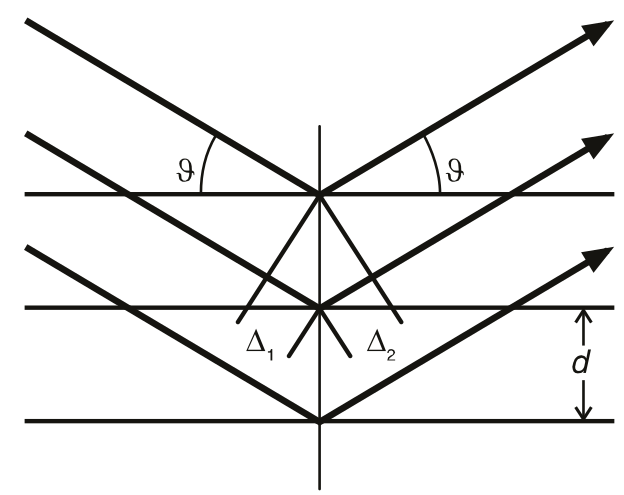
\includegraphics[width=0.35\textwidth]{media/bragg.png}
  \caption{Diagram of the reflection of x-rays at the lattice planes of a
    monocrystal.
    $\Delta_1$, $\Delta_2$: path differences,
    $\theta$: glancing angle,
  $d$: spacing of lattice planes. \cite{leybold_manual1,leybold_manual2}}
  \label{fig:SetupAir}
\end{figure}

